% !TeX encoding = UTF-8
% !TeX root = MAIN.tex

%%%%%%%%%%%%%%%%
\chapter{Introduction}

Artificial Intelligence (AI) has undergone rapid development in the last few years. In today's modern era of mobile phones and computers, algorithms are used on a daily basis to have quick access to information and improve the efficiency of daily life.

While various algorithms (e.g.: Decision Trees, Linear Regression, Support Vector Machines, etc.), which are comprehensible by design, have been developed, the spotlight has turned to Deep Neural Networks (DNNs). This shift is attributed to the increase in computational power and the exponential increase in accessible data. Despite their remarkable accuracy, Deep Neural Networks remain opaque black boxes, which we struggle to understand \cite{Samek_2019}. Nevertheless, the immense improvement in performance and their ability to handle massive datasets have led to widespread adoption in contemporary devices \cite{zhang2022ai}. It is predicted, that algorithms based on Neural Networks will be becoming increasingly popular in the next years.

However, one of the primary difficulties with Neural Networks is the lack of reliable interpretability techniques. Understanding of the models is needed for various reasons: Regulatory laws require the understandability of the data. The deficiency of interpretability in machine learning models leads to the presence of biases, such as gender discrimination and racial disparities. In the absence of a thorough understanding of a model's working, it becomes exceedingly difficult to confirm the functionality. This leads to users not trusting and avoiding machine learning systems. Beyond those user-centric advantages, it also supports the model development process and allows experts to extract valuable insights \cite{Samek_2019}.
 
Numerous interpretability methods have been developed, yet a universally reliable method remains missing. Particularly in the domain of image analysis, encompassing critical applications like automated driving and facial recognition, no solution is present. The decision-making rationale of neural networks remains unclear, attributed to factors like background elements, peripheral objects or lighting conditions. Efforts to address this issue have given rise to several gradient methods, aiming to assign significance values to pixels and represent their importance on neural network decisions \cite{Samek_2019}.

Another alternative option to mitigate the black-box nature of algorithms involves employing model-agnostic methods. These methods offer a computational linkage between features and labels, irrespective of which model is used. Although highly effective for smaller datasets, they begin to struggle as the data size and complexity increase. Because of this, they do not offer a reliable method to quickly make Neural Networks interpretable \cite{molnar2022}.

In light of these prevalent problems, the object of this thesis is to recapitulate interpretability methods for neural networks in computer vision. Emphasis is placed on the evaluation of post-hoc interpretability techniques, forecasting potential future developments and focusing on the strengths and weaknesses of distinct techniques. Concluding the theoretical segment, a practical demonstration showcasing the application of RemOve And Retrain (ROAR)\cite{hooker2019benchmark} is shown. 

\section{Structure of the Thesis}

\begin{enumerate}
	\item In the first chapter \ref{sec:MLandI} "Machine Learning and their Interpretability", an overview of contemporary machine learning algorithms is made, categorizing them into two main groups: algorithms with inherent interpretability and those without. The goal is to make clear how supervised methods can be applied to image recognition tasks.
	\item In chapter \ref{sec:IoNN} "Interpretability of Supervised Machine Learning Algorithms in Image Recognition" we dig into interpretability, emphasizing global and local model-agnostic techniques. These methods offer insights into overall model behaviour, regardless of algorithm specifics. 
	\item In subsequent sections \ref{sec:saliency} "Neural Network specific Interpretability Methods", model-specific post-hoc methods for Neural Networks are introduced. Feature visualization and gradient-based methods are explained.
	\item In chapter \ref{sec:evaluation} "Evaluation of post-hoc Interpretability methods", we focus on evaluating post-hoc interpretability methods. Various approaches to assess the effectiveness and dependability of these methods in offering meaningful insights into intricate models are introduced and discussed. Additionally, the advantages and disadvantages of these approaches are carefully examined to provide a comprehensive understanding of their applicability.
	\item In chapter \ref{sec:summary} "Which evaluation method and attribution method to use?", a conclusion is presented and advice on which evaluation method to use is given. 
	\item In the last chapter \ref{sec:project} "Reconstructing ROAR", the practical application of the ROAR methodology using the Food-101 dataset \cite{bossard14} and MNIST dataset \cite{deng2012mnist} is presented to exemplify the discussed concepts. This real-world instance illustrates the current state of art of evaluation techniques in image recognition.
\end{enumerate}

%%%%%%%%%%%%%%%%
\chapter{Machine Learning and its Interpretability}
\label{sec:MLandI}

In the rapidly evolving landscape of machine learning, interpretability has emerged as an important concept. Before going in-depth into various algorithms and methods, the fundamental question of: "What is interpretable Machine Learning (IML) and why do we need it?" is answered.
\\
A broad definition of IML given by \cite{allen2023interpretable}: "Interpretable machine learning is the use of machine learning techniques to generate human-understandable insights into data, the learned model, or the model output." Interpretability is important for various reasons. Allen\cite{allen2023interpretable} summarizes several objectives for interpretable machine learning: 
\\\\
\textbf{Model Validation}: Interpretable models are essential for validating (by a human) whether a learned model behaves as expected and consistently aligns with prior expectations and knowledge about the system.
\\\\
\textbf{Model Debugging}: When unexpected behaviour occurs, finding the reasons for fault is impossible without understanding the system. To debug systems, an inner understanding of the machine learning system is necessary.
\\\\
\textbf{Transparency, Accountability \& Trust}: IML transforms black-box machine learning systems into understandable systems. Without trust and accountability, using them in high-stakes societal applications is not recommendable.
\\\\
\textbf{Ethics}: Machine learning algorithms can be trained on biased data leading to unfair predictions that are discriminatory. To improve the fairness of machine learning algorithms interpretable methods need to be deployed to assess the fairness. 
\\\\
\textbf{Data Exploration and Discovery}: Insights into major patterns, trends, groups, or artefacts of the data are achieved by applying human-interpretable techniques. These data exploration insights influence the data pre-processing and model decisions. 

Before going into detail about the different methods of interpretability an overview of some currently used supervised machine learning methods is given. Unsupervised machine learning is arguably intrinsically understandable, as the goal is to find a structure in the data. \cite{allen2023interpretable} With those examples, the necessity of interpretability for neural networks should be made evident.

\section{Supervised Machine Learning}

In supervised machine learning, there are a range of foundational classification methods. They are briefly introduced and analyzed for their interpretability. This section analyzes the base functionality of each algorithm. Furthermore, the interpretability is evaluated from a human perspective.
\\
The interpretability of algorithms depends on two factors \cite{molnar2022}. When determining the transparency of an algorithm, we evaluate the human interpretability of how the model learns from the underlying structure of the data. Is it possible for a human to understand the implications of the mathematical operations? The second factor is the interpretability of the learned parameters. Understanding the factors of a linear regression model is easy. Grasping the millions of weights in a neural network is impossible.

In this section, we present a selection of frequently employed supervised machine learning techniques. As will become clear in the following subsections, before the rise of Deep Neural Networks, interpretability was predominantly achieved through methods with inherent interpretability.

\subsection{Linear Models}

When predicting outcomes, one of the simplest methods is to use a linear regression model \cite{puntanen2013methods}. This model predicts by adding up n features ($x_n$) multiplied by a respective individual weight ($\alpha_n$). The predictive output $\hat{y}_i$ is calculated:

$$ \hat{y}_i= \alpha_0 + \alpha_1 x_1 + \alpha_2 x_2 +... +\alpha_n x_{n} + \epsilon$$

The alphas $\alpha_i$ indicate the correlation of each feature. The initial coefficient $\alpha_0$ is known as the intercept, signifying the baseline. The noise $\epsilon$ describes the inevitable errors from inherent non-linearity in real-world dynamics or measurement inaccuracies.
\\
To train the model, the MSE-Loss (Mean Squared Error) or the ABS-Loss (Absolute Loss) is applied between the true label $y_i$ and the predicted label $\hat{y}_i$. The goal is to minimize this loss function. 

$$ \text{MSE-Loss} = \frac{1}{n} \sum_{i=1}^{n} (y_i - \hat{y}_i)^2$$
$$ \text{ABS-Loss} = \frac{1}{n} \sum_{i=1}^{n} |y_i - \hat{y}_i|$$
\\
The interpretation of the model is simple. The factors are described through the coefficient matrix. Each feature is distinctive to the model and the weighting is visible in the factors $\alpha_{i}$ (assuming normalization).

$$ \alpha = \begin{bmatrix}
	\alpha_0 & \\
	\alpha_1 & \\
	... & \\
	\alpha_i &
\end{bmatrix}
$$

Although linear models possess comprehensibility, provide a straightforward method for prediction and are inherently understandable, their application is limited to linear relationships and small datasets. In the domain of image recognition, it is not applicable because the features are not linearly correlated.

\subsection{Distance-based Methods}
\label{KNN}
K-Nearest Neighbours (KNN)\cite{Mucherino2009} serves as a classification method by considering the nearest neighbours. 


Assume you have a dataset $D={(x_1,y_1),(x_2,y_2),…,(x_n,y_n)}$ where $x_i$ represents the feature vectors, and $y_i$ represents the corresponding class labels. Each $x_i$ is a point in a multidimensional feature space, and $y_i$ belongs to one of the classes (e.g., $y_i \in [0,1]$ for binary classification). 
Given a new data point $x_{new}$ that you want to classify, KNN works as follows:\\

1. Calculate the distance between $x_{new}$ and all other data points in the training dataset.\\
2. Select the K data points (nearest neighbours) with the smallest distances to $x_{new}$.\\
3. Count the number of data points in each class among the selected KK neighbours.\\
4. Assign $x_{new}$ to the class that has the majority of neighbours.\\

Although KNN's parameters are not interpretable by default, the underlying concept is straightforward: A sample has the same class as samples with similar features. This makes KNN inherently interpretable and makes it a common choice when interpretability is needed. However, KNN encounter difficulties when dealing with many features and larger datasets, therefore using it for image recognition is not recommended.

\subsection{Support Vector Machines}

Support Vector Machines (SVMs) \cite{boser1992training} are used to find a hyperplane that best separates different classes $y_i$ of data points. The primary objective is to maximise the distance between the hyperplane, defined by the weight vector $\vec{w}$, and the closest data points $x_i$ from each class. This is done to ensure that the datasets are separated as much as possible. Because there may be classification errors and noise in the dataset, it is possible to set an initial regularization parameter $C$ to handle outliers.

The optimization problem SVM in mathematical notion:

$$\text{Minimize } \frac{1}{2} \|\vec{w}\|^2 + C \sum_{i=1}^{n} \xi_i$$

$$\text{Subject to } y_i (\vec{w} \cdot x_i + b) \geq 1 - \xi_i, \quad \xi_i \geq 0 \text{ for } i = 1, \ldots, n$$

$\sum_{i=1}^{n} \xi_i$ represents the sum of slack variables ($\xi_i$), which measure how much a data point violates the margin constraint. While maximising the margin, Support Vector Machines (SVM) seek to reduce this sum, minimizing the violations. $ b $ is the bias term, which shifts the hyperplane away from the origin.

SVMs can handle non-linear data through the kernel trick, in which a kernel is applied to the data, transforming it to a different space before computing the hyperplane. However, as the dimensionality increases, SVMs become non-interpretable, making it challenging to visualize and understand the weight matrix. Moreover, SVMs struggle with larger datasets and high-dimensional feature spaces, making them less effective for image classification.


\subsection{Decision Trees}
\label{decision_tree}


Decision trees are a commonly used machine learning algorithm that proves effective in both classification and regression tasks. The reason for their popularity can be attributed to their user-friendly structure, which can handle both categorical and continuous data. A decision tree is made up of three main types of nodes: root, internal, and leaf nodes, which combine to form a representation often depicted as a tree. In figure \ref{fig:Decision_tree}, a decision tree is plotted, where the distribution is shown in the 'value' field, and the classification of the node/leaf is presented in the 'class' field.

\begin{figure}[H]
	\centering
	\includegraphics[width=150mm]{figs/decision_tree}
	\caption[Decision Tree Example]{Decision Tree Example} 
	\label{fig:Decision_tree}
\end{figure}

The classes are separated in each root node by a decision criterion: $F_i$ <= criterion. The Gini impurity is commonly used for calculating the splitting criterion, which aims to best separate the data in the leaf. New nodes are defined until the dataset is perfectly separated. However, this makes decision trees prone to overfitting as the model becomes overly complex and captures noise or random fluctuations in the training data, rather than the underlying patterns or relationships. Consequently, the resulting tree fits the training data exceptionally but does not generalize well to new or unseen data. 

The depth of the tree can be restricted to avoid overfitting. Then, the majority is utilised to assign a label to the leaf. The depth of the tree can be restricted to avoid overfitting. Nevertheless, as the dimensionality grows, determining the depth becomes more and more challenging.

Random forests\cite{ho1995random}, comprise many decision trees and are known to prevent overfitting. However, they tend to be more challenging to interpret because of the use of multiple algorithms. Techniques like SHAP values \cite{lundberg2017unified} or partial dependence plots \cite{PDP} can be employed to make them more understandable.
\\
Gradient boosting like XGBoost \cite{Chen_2016}, LightGBM \cite{Ke2017} and CatBoost \cite{prokhorenkova2019catboost} share similarities with random forests and decision trees, but they assign differential learned weights to each decision. They suffer from the same interpretability issues as random forests. While decision tree-based methods can be applied for image classification, their accuracy tends to be worse than neural networks.


\subsection{Neural Networks}

The rise of neural networks and their powerful predictive capabilities has made them a popular choice for classification tasks. However, as these networks become increasingly complex, the traditional approach of understanding them through weight examination becomes challenging. With the emergence of Convolutional Neural Networks (CNN) in 2012 \cite{krizhevsky2012nn}, neural networks have become state-of-the-art for image prediction.

In a neural network, each neuron calculates a weighted sum of its inputs and applies an activation function to produce an output. This output serves as the input for the subsequent layer. While various neuron types exist, including convolutional and recurrent neurons, foundational neurons are present in nearly all neural network architectures. A visual representation of a simple neural network can be seen in Figure \ref{fig:Neural_Network}.

\begin{figure}[h!]
	\centering
	\includegraphics[width=150mm]{figs/NeuralNetwork}
	\caption[Neural Network]{Neural Network} 
	\label{fig:Neural_Network}
\end{figure}

In this neural network, each circle, except those in the input layer, represents a weight matrix denoted as $w_{j,i}$. Here, 'j' signifies the hidden layer number, and 'i' represents the weight number within that layer. The output of a neuron is determined by summing the products of the inputs $x_{ji}$, their corresponding weights, and a bias term $b_{ji}$, expressed as $y_{(j+1)i} = \sum_{i=1}^{n} w_{ji} \ast x_{ji} + b_{ji}$. If the neuron is not in the output layer, an activation function, such as Sigmoid or ReLU, is applied to $y_{ji}$, transforming it into the new input for the next layer $x_{ji} = f(y_{ji})$. 

Labeled data is used to train a neural network. The prediction error is minimized by calculating the prediction error and the gradients. This is typically done by backpropagation over several epochs until the network can accurately predict new data.

Modern neural networks, such as ResNet50 \cite{he2015deep} comprise over 50 layers and utilize more than a thousand kernels. Although they produce the greatest results, they lack an intuitive explanation of the learned parameters, unlike other types of supervised machine learning algorithms. Nonetheless, interpreting them to some degree is a necessity. Therefore, methods were developed that attempt to make any supervised machine learning algorithm interpretable. 

\chapter{Interpretability of Supervised Machine Learning Algorithms in Image Recognition}
\label{sec:IoNN}

Before going into detail in the chapter, the primary challenge of image recognition is explained: Consider an image with dimensions of 3x224x224. The key objective in achieving model interpretability is to discern which elements of the image are responsible for influencing the model's output. The task is to highlight or establish a clear link between specific regions within the image and the output. This complexity explains why many interpretability methods often prove inadequate for image recognition. For instance, when an object within the image transitions from one quadrant to another, different areas of the image become responsible for the classification. Furthermore, challenges such as image blurriness, mirroring or the presence of multiple potential classifications make interpretability difficult. This process of creating a correlation between image features and classification becomes exceedingly complex and non-understandable for neural networks. Furthermore, the high dimensionality makes the brute-force method too computationally expensive. To address these issues, special model-specific interpretability methods have been developed.\\

Before going into details of interpretability methods for this problem, a framework \cite{allen2023interpretable}, see figure \ref{fig:IML_Overview} is presented for classifying supervised machine learning methods and interpretability methods.

\begin{figure}[H]
	\centering
	\includegraphics[width=100mm]{figs/Overview}
	\caption[Interpretability categorization ]{Interpretability categorization (Figure from \cite{allen2023interpretable})}
	\label{fig:IML_Overview}
\end{figure}

\textbf{Intrinsic vs Post-hoc}: Interpretability methods can be broadly classified into intrinsic and post-hoc techniques. Intrinsic methods are inherently understandable by design, while post-hoc interpretations involve analyzing the model's behaviour after its creation. Typical intrinsic understandable methods are Decision Trees \ref{decision_tree} and KNNs \ref{KNN}. As methods for classifying data become more difficult, the methods themselves become less interpretable and lose their intrinsic interpretability. Therefore, post-hoc methods must be applied to them to make them interpretable again.
\\
\textbf{Global Interpretations vs Local Interpretations}: Global Interpretations encompass the entirety of a fitted model. In contrast, local interpretations zoom in on specific portions of the model landscape, such as class boundaries. Local interpretations exist because for some models it becomes too complex to generate a global interpretation. In order to still have some interpretability in the model, local interpretations are used.
\\
\textbf{Model-Specific Interpretations vs Model-Agnostic Interpretations}: 
Model-specific interpretations are tailored to a particular class of algorithms, like gradient methods for neural networks. Model-specific interpretations make use of the inherent information as weights or gradients in a model. In contrast, model-agnostic interpretations, such as LIME or SHAP, can be applied to any classification algorithm because they do not require model-specific knowledge.

The goal of this section is to present several commonly used interpretability methods and evaluate their suitability for image classifications. As Neural Networks are the best-performing methods for image recognition, the focus lies on the suitability of the interpretability methods for Neural networks. After going over model-agnostic interpretability methods in the next sections, we go in-depth about model-specific interpretations for neural networks in section \ref{sec:nni}. 


\section{Model-Agnostic Methods and their applicability to Neural Networks}

Model-agnostic methods can be applied to any method. However, it does not make sense to use the same method for every algorithm. In this section, global and local agnostic methods are summarised and their applicability to neural networks in image classification is discussed. 


\subsection{Global Model-Agnostic Methods}

Global Methods aim to provide a complete overview of the functioning of a model. However, it is difficult to represent the non-linearity in image classification for multiple classes. While some methods work reasonably well for the computation required, there is no global agnostic method that fully covers the need for interpretability.

\begin{enumerate}
	\item \textbf{Partial Dependency Plots:} Partial Dependency Plots (PDPs)\cite{PDP} display the relationship between individual or multiple features and an outcome. However, when dealing with a bigger feature size, there are too many plots to make sense of the data. Therefore they are not feasible for Neural Networks and image recognition tasks.
	\item \textbf{Accumulated Local Effects:} Accumulated Local Effects (ALE)\cite{apley2019visualizing} are an advancement of PDP. While it overcomes certain difficulties from PDPs, they struggle with the same problem when it comes to a bigger feature size.
	\item \textbf{Feature Interaction:} Feature Interaction analyzes the interaction between features inside the model. The underlying Friedman's H-statistic\cite{friedman2008predictive} is a method to evaluate the correlation and variance. Because of the complexity of image tasks and the high computational costs, this method is not applicable to Neural Networks in a meaningful matter.
	\item \textbf{Functional Decomposition:} Functional Decomposition is used in Neural Networks. In Chapter \ref{sec:network_dissection} a method to disassemble networks is presented.
	\item \textbf{Permutation Feature Importance:} Permutation Feature Importance is regularly used in visual machine learning tasks. In section \ref{pertubation} an example of a perturbation method is shown.
	\item \textbf{Prototype and Criticism:} The creation of clusters using the prototype and criticism method involves categorizing well-presented data instances as 'prototypes' and sparsely presented ones as 'criticism'. This approach aims to improve the interpretability of these clusters by verifying their classification accuracy. However, a significant challenge with this method arises when applying it to images, as it can be difficult to generate reliable clusters that effectively group the data.
\end{enumerate}


\subsection{Local Model-Agnostic Methods}

The aim of local model-agnostic methods is to reveal knowledge of how individual cases of a model behave. In the field of image classification, where non-linearity and multiple classes contribute to added complexity, achieving accurate interpretability for a single class is already challenging. Although some techniques effectively manage the trade-off between computational efficiency and interpretability in certain scenarios, there is currently no universally accepted model-agnostic method for achieving this. Nevertheless, they can be applied to Neural Networks and potentially give meaningful interpretations.

\begin{enumerate}
	\item \textbf{LIME: Local Interpretable Model-agnostic Explanations:} LIME\cite{ribeiro2016should} generates explanations in a local scope by training interpretable models on the predictions of a model. LIME only covers a single local context of the model. LIME can be applied to various types of data, including image data.
	\item \textbf{Scoped Rules (Anchors):} Anchors \cite{ribeiro2018} are distinctive patterns or conditions which guarantee a prediction. Finding anchors becomes increasingly expensive with more features present and is not normally used in neural networks. 
	\item \textbf{Individual conditional expectation curves:} ICE \cite{goldstein2014peeking} display one line per data sample and display how the sample changes when a feature changes. It is an individual version of PDP. It is not used in image classification or to evaluate neural networks.
	\item \textbf{Counterfactual explanations:} Counterfactual explanations \cite{wachter2017counterfactual} of a prediction explain the smallest change of feature values which is necessary to change the prediction of an output. The problem in using this method is that for each instance multiple counterfactual explanations exist. The use of counterfactual explanations in image recognition as a standalone method is not common.
	\item \textbf{SHAP (SHapley Additive exPlanations):} SHAP values \cite{lundberg2017unified} calculate how much each feature contributes to the difference between a models prediction for a specific instance and the average prediction across all instances. Positive SHAP values indicate features that increase the predicted likelihood for a particular class, while negative values indicate features that decrease it. It is used commonly in neural networks.
\end{enumerate}

While the summarized techniques can be applied to neural networks, they do not provide a universal solution for interpretability. For this reason, Model-specific methods for neural Networks were developed which make use of the inherent parameters of neural networks.

\section{Model-Specific methods for Neural Networks}
\label{sec:nni}
In the domain of Natural Language Processing (NLP) and Computer Vision, Deep Learning has proven very successful. By passing the features through a sequence of layers, characterized by matrix multiplications with kernel weights and nonlinear transformation functions, a prediction is computed. Depending on the specific task, additional elements like Long Short-Time Memory(LSTM) layers and Convolutional layers are utilized. Given the immense amount of mathematical operations and the non-linearity underlying a single prediction, humans are not fit to apprehend the mapping. To interpret predictions, we would have to decipher the intricate learned knowledge of numerous different kernels and weights.
Recognizing that humans cannot grasp millions of weights, the demand for interpretability methods is high. To assess the behaviour and predictions of Deep Neural networks, specific interpretability methods were developed. These methods calculate the likelihood of a feature being responsible for the result.
\\\\
While model-agnostic methods offer an approach to understanding Neural Networks, the sheer size of the data used to train and test Neural Networks makes this task difficult. For instance, in an image with the dimensions of 3x224x224, as commonly encountered in Food-101, the data features exceed 150.000. In NLP tasks, where vocabularies often encompass around 20,000 words, the computational complexity renders most model-agnostic techniques as too expensive.
\\
In the pursuit of comprehending the complexity of Deep Neural Networks, it makes sense to utilize the weights and gradients in the model. The information saved in the hidden layers as learned weights can be used to evaluate the network. Moreover, the gradients can be taken into consideration as well. In the following subsections, several concepts for understanding Deep Neural Networks are introduced. 

\subsection{Feature Visualization}
\label{sec:network_dissection}

Feature Visualization aims to make parameters in singular layers in neural networks understandable. The goal is to give an understanding of a deep neural network by dissecting each layer and understanding the underlying parameters through visualization.

The higher-level features in these networks relate to clear concepts, shown in Figure \ref{fig:feature-visualization}. As the features (image-pixels) pass through the layers, the resembled structure changes at each layer. In each convolutional layer, the network gains new and more complex features. The joining of fully connected layers then converts image-based data into predictions.
\\
\begin{figure}[H]
	\centering
	\includegraphics[width=170mm]{figs/FeatureVisualization}
	\caption[Network Dissection: Feature Visualization ]{Network Dissection: Feature Visualization (Figure from \cite{olah2017feature})}
	\label{fig:feature-visualization}
\end{figure}

The figure visualizes this process. The first convolutional layers find simple features like edges and basic textures. Later, they recognize more detailed patterns. The deepest layers learn about parts and objects. This object information passes to the other hidden layers, which then finally make a prediction.

Feature visualization is based on activating one kernel in the network. This involves maximizing the activation of a specific neuron (Visible in figure \ref*{fig:optimization}). There are two methods for achieving this. First, we can make use of the training image that triggers the highest activation. Yet, this approach faces a significant problem. When an image contains multiple objects, it is hard to pinpoint which object causes the activation. Because of this, an alternative route is adopted: generating new images from random noise. This is accomplished through methods like Generative Adversarial Networks (GANs) \cite{goodfellow2014generative} or other diffusion-based techniques\cite{zhang2023survey}.

\begin{figure}[H]
	\centering
	\includegraphics[width=170mm]{figs/ab}
	\caption[Activation Maximization]{Activation Maximization (Figure from \cite{olah2017feature})}
	\label{fig:optimization}
\end{figure}

Feature visualization provides a first insight into the behaviour of a model, improving the understanding of its inner layers. It also has the potential to enrich domain understanding by aligning learned features with domain-specific knowledge. Furthermore, it can assist in debugging and refining models, contributing to their overall performance improvement. However, interpretation of the visualized features is difficult and decision making is challenging to understand.

\subsection{Network Dissection}

Network dissection, a technique introduced by Olah in 2018\cite{olah2018the}, builds on the principles of feature visualization. This method establishes a link between individual kernels and the prediction of specific features by exploiting the concept of visualizing the importance of channels and kernels, as introduced in the previous section. For each kernel, the predicted classifier is displayed in a percentage.

Although this method is effective in comprehending low-level features, comprehending high-level features remains a challenge. Furthermore, analyzing a single sample is very time-consuming. However, this interpretability technique holds significant potential for enhancing the transparency of neural networks.


\section{Attribution Maps}
\label{sec:saliency}
Attribution maps are visualizations that highlight the regions of an input image that have the most significant impact on a model's output. By revealing the areas that strongly influence a prediction, saliency maps bridge the gap between the model's "black-box" nature and human understanding. An example attribution map is visible in figure \ref{fig:saliency}.

\begin{figure}[H]
	\centering
	\includegraphics[width=150mm]{figs/SaliencyExample}
	\caption[Attribution Map]{Attribution Map: Classification of a swan (Figure from \cite{captum})}
	\label{fig:saliency}
\end{figure}

Attribution maps are typically calculated using SHAP\cite{lundberg2017unified} or gradient methods. Attribution maps provide a direct and intuitive way to understand which parts of input data influence a model's decision. The main difficulty is in generating reliable attribution maps. Kindermans \cite{Kindermans2019} shows that attribution methods can be highly unreliable. The remaining subsections introduce some commonly used methods. The key objective for all the following methods is the same: Generating a reliable and easily understood attribution map.

\subsection{Visualizing Image Classification Models and \& Deconv-Net}

Visualizing image classification models (Vanilla Gradient) \cite{simonyan2014deep} focuses on computing gradients within neural networks. It involves generating a forward pass of an image and then computing gradients for the class scores. These gradients are then visualized. However, this method faces two challenges. First, when Rectified Linear Units (ReLU) are used, negative gradients are seen as unimportant and are set to zero. This leads to an information loss in the gradients. Second, in pooling layers, gradients are absent.
\\
The Devonc-Net from Zeiler \cite{zeiler2013visualizing} addresses these problems:
A Deconv-Net-layer \cite{Zeiler2011AdaptiveDN} is attached to each convolutional layer providing a path back to the image pixels. The Devonc-Net learns weights to reverse the process from input to the last convolutional layer. Unpooling in Deconv-Net addresses the non-invertibility of pooling operations by preserving the original maxima locations through switch variables, which are used to reconstruct the activations. To maintain positive signals during reconstruction, a reverse ReLU non-linearity is applied in each layer, similar to the forward pass. Additionally, Deconv-Net utilizes transposed filters, effectively mirroring each filter both vertically and horizontally to achieve filtering in the reverse direction.

This makes it possible to highlight the responsible features for a classification output.

\subsection{Gradient-weighted Class Activation Map (Grad-CAM)}

Grad-CAM \cite{springenberg2015striving} ignores low-relevancy classes, which means that percentages for predictions below a certain threshold are not taken into account. The method then backpropagates gradients specifically for the classes of interest. These gradients are rescaled to fall within the [0,1] range and visualized. Grad-CAM takes into account all layers except for the convolutional layers. Evaluating the importance of each kernel prior to the convolutional layers provides insight into the importance of each input feature. This leads to a coarse accuracy, as pooling layers and convolutional layers are not handled and the resolution is up-scaled to the required format.

\subsection{Guided Grad-CAM}

Guided Grad-CAM combines the backpropagation \cite{springenberg2015striving} with another method to have a better localization. The up-sampled attribution map from Grad-Cam is multiplied pixel-wise with another attribution method. This acts as a lens for other attribution methods to focus on specific parts of the attribution map.

\subsection{Integrated Gradient}
\label{IG}
Integrated Gradient \cite{sundararajan2017axiomatic} computes the integral of the gradients of the model's prediction with respect to its input variables. By integrating over this path, it quantifies how each feature contributes to the change in the model's prediction. A reference variable, such as a baseline is used to measure how each feature influences changes in each prediction. The method is commonly used because it is applicable to any model and achieves good results.

\subsection{Ensemble Methods: Smooth Gradient, Smooth Grad² and VarGrad}

All the following methods can be applied to gradient-based techniques to adjust their behaviour and enhance their robustness in various applications.

\text{SmoothGrad} \cite{smilkov2017smoothgrad} is a smoothing approach to mitigate noise in gradient calculations. To achieve this, it generates a set of J noisy estimates by independently adding Gaussian noise $\theta$ to the input $x$. These noisy estimates are then averaged to obtain a more reliable and accurate gradient estimate, as represented by the formula. $g$ is describing the calculation of an attribution map, $A$, is the attribution map:

$$ A = \frac{1}{J}\sum_{i=1}^{J} (g(x+\theta))$$

\text{SmoothGrad²} \cite{hooker2019benchmark} builds upon the concept of SmoothGrad by squaring all estimates before averaging them. This modification is aimed at emphasizing the contributions of gradients while further reducing the impact of noise. The formula is as follows:

$$ A = \frac{1}{J}\sum_{i=1}^{J} (g(x+\theta)^2)$$

\text{VarGrad} \cite{adebayo2020sanity} offers an alternative approach to aggregating gradient estimates. Instead of summing them up or averaging them, VarGrad focuses on estimating the variance of these estimates. This aggregation provides insights into the variability of gradient information across different perturbations, offering a unique perspective on the model's behaviour. The formula for VarGrad is expressed as:

$$ A = Var(g(x+\theta))$$


%\subsection{Excitation Backpropagation}
%
%Excitation backpropagation\cite{zhang2018} focuses on a set of neurons within a neural network during the computational process. By doing so, it enables the combination of gradient information with the attribution maps, leading to precise object localization.
%
%The key feature of excitation backpropagation is the use of a probabilistic Winner-Takes-All (WTA) formulation. This formulation produces normalised attention maps, allowing for direct subtraction of these attention maps. This subtraction operation is crucial for highlighting the regions of interest within the neural network's activation, making it easier to understand which parts of the input data contribute most to a particular decision or classification.
%
%\begin{figure}[h!]
%	\centering
%	\includegraphics[width=150mm]{figs/TopDown}
%	\caption[CNN classifiers top-down attention map]{CNN classifiers top-down attention map \cite{zhang2018}}
%	\label{fig:topdown}
%\end{figure}
%
%The concept of identifying task-relevant neurons is central to Excitation Backprop. This involves evaluating the relative likelihood of a neuron "winning" against others within the same layer. Neurons with higher winning probabilities are deemed more relevant to the task at hand, and this information can be leveraged to understand the network's decision-making process and to localize objects or features within the input data.


%\begin{figure}[h!]
%	\centering
%	\includegraphics[width=150mm]{figs/DeterministicWTA}
%	\caption[Identifying task-relevant neurons in the network.]{Identifying task-relevant neurons in the network. The red shading of a dot indicates its relative likelihood of winning against the other ones in the same layer. \cite{zhang2018}}
%	\label{fig:taskrelevant}
%\end{figure}

\subsection{Summarizing Attribution Maps}

There exist many more attribution maps but there exists one major problem: There is no consensus on which method should be used. While attribution maps have advantages \cite{molnar2022}, such that they are fast to compute and easy to interpret, they are also unreliable and can be insensitive to models and data. Furthermore, it is difficult to know whether an explanation is correct. In the next chapter, the evaluation of interpretability methods is discussed.

\newpage

\chapter{Evaluation of post-hoc Interpretability Methods}
\label{sec:evaluation}


This chapter discusses the evaluation of attribution maps and the underlying gradient methods. Finding appropriate evaluation methods for attribution maps is difficult. A significant challenge is the lack of ground truths in attribution maps. Nevertheless, several evaluation methods have been developed that attempt to assess the performance of saliency methods. While they do not provide an objective truth as to whether one saliency method outperforms another in all tests, they can provide some indication of the effectiveness of saliency methods. Gupta\cite{gupta2022new} suggests that these evaluation methods can be broadly categorized into two types:

\textbf{Extrinsic Evaluation}: 
The evaluation is compared against predefined ground truths explanations, established by a human annotator or by another network e.g.(\cite{zhang2018}). However, the sheer amount of images makes the evaluation challenging. Furthermore, the quality of an attribution map is hard to judge. When is an evaluation correct? Also, Adebayo \cite{adebayo2020sanity} underscores the issue of confirmation bias, where an explanation may be considered correct because it highlights the same regions as humans might choose, but it is not sure that the model employs the same learned concepts. 

\textbf{Intrinsic Evaluation}: 
Intrinsic methods rely on computational analyses within the neural network itself, without requiring human judgments. These methods are based on creating a new composite input using the heat map and the original input. Then they are evaluated using either the same model\cite{dabkowski2017real} or new models are trained and evaluated\cite{hooker2019benchmark}. While both these methods generate meaningful results, they do not offer an objective evaluation method. Without re-training it is not clear if the degrade in performance stems from the distribution shift or the removal of informative features \cite{hooker2019benchmark}. By re-training the model, a different model is evaluated. 
\\

Many interpretable AI methods exist and comparing their effectiveness is difficult. Neely, \cite{neely2021order} has tested several explainable AI methods in the domain of NLP and can only find little correlation. Additionally, the correlation is model and task-dependent, which furthermore weakens this assumption. However, it is unclear whether this result holds for image classification.
\\
After considering all these facts, it is not possible to meaningfully evaluate saliency methods by comparison or without violating fundamental assumptions. In the upcoming sections, potential evaluation metrics and methodologies are introduced to provide a more meaningful assessment. These metrics and methods do not fundamentally solve the problems, but they offer some guidance for evaluation.
\\
It is to note, that in evaluation the composite input of the image $x \circ A$ is often used. It describes an image with some parts of the pixels replaced by a gray value or the mean value, to hide the information of specific pixels. The pixels are chosen according to the highest or lowest values in the attribution map. Those new inputs are then measured using intrinsic methods. The hypothesis is: If the not removed pixels are not important and the original net outputs the same labels, then the removed pixels are not important. This hypothesis proves difficult in the domain of CNN's, as the composite input of various pixels is used. 

\section{Completeness and Soundness}

Gupta, 2022 \cite{gupta2022new} proposes Soundness and Completeness, which proposes metrics to evaluate the effectiveness of evaluating composition methods.

Soundness: A certain part of the image is responsible for the output of the classifier. Some parts of the pixels are responsible for the classification of the label. In practice, this means that if you apply any mask to the image that still makes the x\% of the most important pixels visible, then the classification will be the same. This also means that if some of these important pixels are not visible, then the confidence of this classification will decrease. \\
Completeness: No matter what mask is chosen, as long as the x\% most important pixels are visible, the classification is correct. In practice, this means that when the important pixels are visible, the classification remains correct, regardless of the appearance of the other pixels.\\

These two metrics are useful for evaluating the correctness of masking. However, it is only one metric for other evaluation frameworks. Gupta suggests that intrinsic evaluation methods should test for both completeness and soundness.

\section{Evaluating the Visualization of What a Deep Neural Network has learned}
\label{pertubation}

In the paper by Samek\cite{samek2017} a method is described, where the most important pixels detected by an attribution method are systematically replaced with randomly sampled values using a greedy algorithm. The objective is to measure the impact on the classification value f(x). The method can be applied by only removing the important pixels or by defining a local neighborhood around the pixel which is replaced as well. This neighborhood is defined because, from the context of the nearby pixels, the same information can be deduced.

While the method produces results which confirm that removing important pixels leads to a performance drop, the models are not retrained. This leads to an evaluation of a different data distribution and violates the assumption of a similar data distribution for the train and test data.

\section{A Benchmark for Interpretability Methods in Deep Neural Networks }

This paper \cite{hooker2019benchmark} presents two methods for numerically evaluating attribution maps. "RemOve And Retrain (ROAR)" and "Keep And Retrain (KAR)". This is done by removing supposedly informative features from the input and observing the response of the neural network. The section \ref{sec:project} gives an example of a practical application for MNIST\cite{deng2012mnist} and Food-101\cite{bossard14}.


ROAR can be applied to any method that produces attribution maps. It identifies 10, 30, 50, 70 or 90 \% of the most important pixels in an attribution map and ranks them according to their numerical importance. In order to have a baseline against which to compare, a random baseline is generated which randomly assigns the importance of the pixels.\\ After the most important pixels have been identified, new datasets are generated for each threshold. In this step, x\% of the most important pixels are replaced by the mean value of the data set.\\
Once the new data sets have been generated, new uninitialized models with the same architecture and learning parameters are trained on this modified data set. The same train/test split should be used as for the original model. This is done for several runs to ensure consistency of results.
After retraining for each set of removed pixels and attribution maps, the results are compared. A random baseline should have a slower loss of accuracy than an attribution map.

KAR works in a similar way to ROAR, but instead of removing the most important pixels, it removes the least important pixels. As KAR performs worse than ROAR, it is not described further.\\
\\
The conclusion of Hooker \cite{hooker2019benchmark} is that some commonly used attribution estimators like Gradient\cite{simonyan2014deep}, Integrated Gradient\cite{sundararajan2017axiomatic} and Guided Backpropagation\cite{springenberg2015striving} perform worse than random assignments in ROAR. On the other hand, the effectiveness of Smooth-Grad-Squared and VarGrad was confirmed. However, ROAR is sensitive to the dataset used. While it does provide a numerical evaluation, it is sensitive to the model and dataset used and therefore cannot universally evaluate an algorithm.

\section{Benchmarking Attribution Methods (BAM)}
\label{sec:bam}

As already mentioned before, determining the ground truth of an attribution map is impossible. However, it is possible to compute the relative importance of specific features when comparing it between two different models\cite{yang2019benchmarking}. BAM\cite{yang2019benchmarking} uses this to evaluate different attribution methods.
\\
Visualize an image consisting of two distinct pixel sets:\\ 
Each image contains one object, represented by the $p_o$ pixels, and the remaining pixels $p_s$ make up the background scene. By training two distinct classifiers, one trained to detect objects and the other trained for scene identification, we expect that the relative feature importance for the $p_o$ pixels should be higher for the object classifier than for the scene classifier. Conversely, the same holds for the $p_s$ pixels for the scene classifier.\\
In BAM, such image-scene pairs are created systematically. To address the distribution shift problem, objects with a mean similar to the mean of the dataset are chosen so that they do not significantly alter the image distribution. Attribution maps are calculated for each image and both trained classifiers. Those attribution maps are then compared using different metrics. However, the results show different results for various metrics and no clear result can be given for any method.\\
The advantage of BAM over ROAR \cite{hooker2019benchmark} and other methods is the lower computational cost. No retraining or perturbation is required. However, the method has the usual problems of evaluation algorithms: sensitivity to the dataset and model and not offering a universal truth.


\section{Sanity Checks for Saliency Maps}

Adebayo \cite{adebayo2020sanity} proposes two "sanity" tests to evaluate whether attribution methods are meaningful. It reveals that visual inspection by humans does not determine if the explanation is sensitive to the underlying model and data. Two instances of the framework are tested:
\\
The model \textbf{parameter randomization test} involves comparing the output of a saliency method on a trained model with the output of a randomly initialized untrained network of the same architecture. The output should differ, otherwise, the saliency map is considered ineffective. An example of this test is visible in figure \ref{fig:Sanity}. The \textbf{data randomization test} randomly shuffles the labels of the data. Afterwards, the model is trained on the altered dataset. If the saliency maps do not differ from a normally trained model, then the method does not depend on the relationship of the images and labels.\\
\begin{figure}[H]
	\centering
	\includegraphics[width=150mm]{figs/Sanity}
	\caption[Cascading Randomization on Image Net]{Cascading Randomization on Image Net. The figure shows the original explanations. Progression from left to right indicates complete randomization of network weights up to that block inclusive. The last block corresponds to a network with completely reinitialized weights. (Figure from \cite{adebayo2020sanity})}
	\label{fig:Sanity}
\end{figure}
If either of these two hypotheses fails during testing, the method under evaluation can be rejected, indicating that it fails a critical sanity check. On the tested methods, Guided BackProp \& Guided GradCAM fail these sanity checks.


\chapter{Concluding Thoughts on Attribution and Evaluation Methods}
\label{sec:summary}
Numerous attribution maps and possible evaluation methods have been looked at and it leaves data scientists with one question: Which evaluation method and attribution method should be used?
\\
The unsatisfactory answer is: We do not know. Depending on the model and dataset used, different evaluation methods give varying outcomes. In Sanity check by Adebayo \cite{adebayo2020sanity} and ROAR by Hooker\cite{hooker2019benchmark} some methods were seen as unsuitable for the task considered. However, this was dependent on the model and the dataset. Considering there exists no ground truth for an evaluation method, there also is no ground truth for the attribution method. Opting for an SG - GRAD or a VAR-GRAD approach might result in favourable results for ROAR and Sanity checks. However, it remains difficult to evaluate visual explanations and there is no established ground truth to determine which evaluation method is the best. Consequently, further research is required to provide clearer guidance in this area.

%%%%%%%%%%%%%%%%
\chapter{Reconstructing ROAR} % 4 pages
\label{sec:project}

\section{Scientific Motivation and Goal}

After looking at different methods in theory, we look at one approach in detail. We decided to look at ROAR\cite{hooker2019benchmark} because it is a relatively recently published study. We try to reproduce some of the experiments. Only a small part of the original experiment was reconstructed because the complexity and the required computing power were not available. In addition, we also want to look at the fluctuations between the different runs, as these were not included in the original paper.


Due to resource constraints, the research was limited to evaluating Food-101 \cite{bossard14} using two interpretability methods along a baseline model. Instead of five control runs, only four were performed. As an initial proof of concept, the evaluation was performed on the MNIST dataset\cite{deng2012mnist}.


\section{Graying out Pixels}
\label{gray}
In ROAR, pixels are grayed out to hide potentially informative pixels. Graying out pixels does not necessarily mean that the information is completely hidden. To provide a theoretical explanation for the implications of removing input dimensions on the resulting accuracy, the following two factors\cite{hooker2019benchmark} should be considered:

\begin{enumerate}
	\item Input dimensions are removed and the accuracy of the model drops:\\ The removed input was informative for the model and their absence reduces the ability of the model to identify the correct class.
	
	\item We remove inputs and the accuracy of the model does not drop.\\ (a) It is possible that the removed input dimensions were not important for the model’s decision-making process. The attribution map failed to identify important features, such as background pixels. (b) The input could be redundant and the information can be reconstructed using other available inputs. 
\end{enumerate}

Removing pixels in RGB images can create new patterns for models to predict. Therefore, human assumptions about the effect of removing pixels should be made only after careful consideration.


\section{Project Setup MNIST}
\label{sec:MNIST}

A. Choice of the MNIST dataset

Before starting a large computation on the Food-101 dataset, the method was tested on a smaller dataset (MNIST) and with only one interpretability method to test the programmed pipeline. The MNIST dataset consists of 10 classes and 70,000 different images. The images are 28x28 pixels and a pixel has a value in the range [0,1] in greyscale. It was chosen because it is a small dataset and the reconstruction of the method can be achieved easily. Furthermore, the dataset is only 50 MB in size and a model can be trained without significant computational effort. For the proof of concept, only integrated gradient \cite{sundararajan2017axiomatic} and a random baseline were computed.

B. Training the model

The model used in this report is a convolutional neural network architecture consisting of two convolutional layers, two pooling layers, and three linear layers. The model was trained for ten epochs with a learning rate of 1e-3 and an SGD optimizer with a momentum term of 0.9. The batch size was 64. Across five separate runs, the model achieved an average accuracy of $97.4\%\pm0.4\%$ on the test data.

C. Dataset preparation and Splitting

The dataset used in this report was normalized using the mean and standard deviation and was split using the PyTorch library's default splitting method (60,000 images for the training data and 10,000 images for the test data). This split has a fixed test and train set which includes a homogeneous distribution of the classes. The training data was shuffled randomly for the training runs. The cross-entropy loss was selected for training runs. The same dataset split was used for all training runs to ensure consistency in the results.

D. Example of the modified dataset

The modified dataset is the result of combining the attribution map with the original image pixels $A \circ p$. In this operation, the most x\% important pixels are replaced with the mean value of the dataset. In figure \ref{fig:IGvsRandom} the difference between the two altered datasets is visible. In the first row, the random baseline is visible, and in the second row, the Integrated Gradient evaluation is shown. 10, 30, 50, 70 and 90\% of the pixels are grayed out (left to right).

\begin{figure}[H]
	\centering
	\includegraphics[width=120mm]{figs/IGvsRandom}
	\caption{Integrated Gradients and Random Baseline Comparison}
	\label{fig:IGvsRandom}
\end{figure}

Judging by human intuition, Integrated Gradients \cite{sundararajan2017axiomatic} seems to block out information more reliably. The model is expected to perform worse after retraining. However, human intuition can be problematic in neural networks as mentioned in section \ref{gray}.

E. Retraining on the new datasets

To ensure that the model learns consistently, the same split and learning parameters as in the standard case were used to retrain the model on the newly modified dataset. An untrained network was created and then retrained for each training run. To validate the results and to minimize the effect of random seed initialization, the training was performed with 5 different seeds and 5 independent models were created. The exact results can be found in the appendix.

F. Advantages and Disadvantages of the setup

Due to the small size of the dataset and the limited number of classes, training a model is fast and effective. A disadvantage is the limited venerability of this setup to other datasets and models. The majority of use cases primarily involve working with images in the RGB colour space, using deep learning models that are often more complex. In addition, RGB images combine 3 channels, making attribution maps more difficult to compute and understand.

G. Results

\begin{figure}[H]
	\centering
	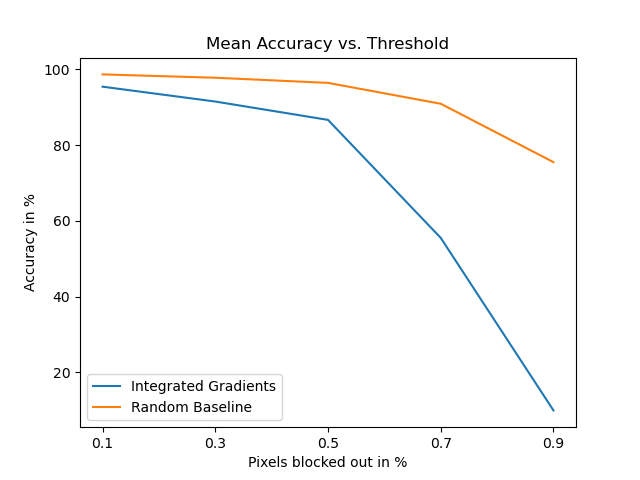
\includegraphics[width=100mm]{figs/mean_accuracy_vs_threshold}
	\caption{Accuracy: Random Baseline and Integrated Gradient}
	\label{fig:Accuracy}
	
\end{figure}

Figure 6.2 shows the decay in the accuracy of the random baseline and the integrated gradient. Integrated Gradient seems to have a faster information decay, and at 90\% of the grayed-out pixels, the classification is 10\%, which is the same as a random classification. Note that Integrated Gradient has a very high standard deviation at 70\%. This is because two control runs happened to learn a random classification, while the other three still managed to learn a classification. In this experiment, Integrated Gradient seems to identify more informative pixels than the random baseline for the MNIST dataset. \\
One possible explanation for this result, which differs from that of the ROAR experiments, is that for simple models, such as the one used in this experiment, and for simple data sets, such as the MNIST data set, it is easier for attribution methods to find informative pixels. Furthermore, the structure of a gray-scale image is easier than an RGB image.

\section{Project Setup Food-101}

After building a functional, fast pipeline for the ROAR algorithm, some of the experiments of the original paper were reconstructed. Originally, the goal of the thesis was to reconstruct Image Net. However, the computation time was too long with the available setup, so Food-101, which has only about 5 GB, was chosen.

A. Training the model

The model used in this report is ResNet50 \cite{he2015deep}. The Food-101 \cite{bossard14} dataset was chosen for replication. The learning rate was set to 0.175 and the batch size was set to 64. Using an SGD optimiser with momentum of 0.9, weight decay of 0.0001 and a scheduler at epoch 30 with gamma=0.1, an average accuracy of $70.5\% \pm 1.6$ was achieved over 5 separate training runs on the test score (no validation split was used). Cross-entropy loss was used. A total of 31 epochs were run. By using this particular training setup, the model learns more about the specific data in the last epoch. In the last epoch, an accuracy of 95\% was achieved on the training data.\\
In the original paper, an accuracy of 84.54\% was achieved on the Food-101 dataset. A lower accuracy was achieved because different training parameters were used in our experiment. We used a smaller batch size of 64 instead of 256 and fewer epochs, 31 instead of 90. More fine-tuning could have been done to achieve a better test score, but the results were considered good enough for our experiments.

B. Dataset preparation and splitting

The data was resized using centre-crop to make all images 3x224x224. They were then normalised. No data enhancement such as flipping and mirroring was applied. The standard 75:25 split was used. In the original dataset, the training and test data have a fixed split, which we also used for this report. The saliency maps used to generate the datasets were computed using a single model. The original paper does not clearly state how the pixels are replaced. In these experiments, the input layers were considered as 3x224x224 maps and each channel of a pixel was replaced individually by the mean of that channel.

C. Retraining the models

The same procedure was followed as in the MNIST section \ref{sec:MNIST}. However, only 4 control runs were performed instead of 5. The exact results can be found in the Appendix.

B. Results

\begin{figure}[H]
	\centering
	\includegraphics[width=160mm]{figs/Acurracy Plots}
	\caption {Comparison of the accuracy behaviour of the original model vs the modified model.}
	\label{fig:food101Res}
\end{figure}

Figure \ref{fig:food101Res} shows the accuracy of the retrained models in the original paper and the accuracy of our retrained model. Our experiments confirm the results of the original paper for integrated gradient and guided backpropagation. The random baseline seems to block out more important pixels than the other attribution methods. The fact that the accuracy drops so slowly makes it unclear whether the method can be used to reliably test attribution methods. While our accuracy drops more quickly, this is probably due to the different training setups. The standard deviations are small and it appears that the results can be replicated consistently.

\section{Summary and Interpretation}

The main idea of ROAR was confirmed using MNIST as an example. For simple datasets such as MNIST, the concept can be shown to be meaningful. However, the performance of interpretability methods seems to vary for different datasets and models. This sensitivity to the dataset and the model makes it difficult to judge what is causing the result. It could be the attribution method, the dataset, the model, or the specific training setup of the model. It is difficult to make a clear statement.

Findings and critique:

1) Choosing a different model and dataset as well as a different training setup changes the results. 

2) Different results are obtained depending on the attribution method chosen in the original paper. What ROAR does with ensemble methods is to remove patterns that are important to the model. However, this may be due to the facts mentioned in section \ref{grey}. Ensemble methods may be able to remove larger clusters and their neighbours, resulting in a greater loss of patterns. When some important pixels are removed, other neighbouring pixels may improve in performance because they suddenly carry the important information. However, it is still unclear what exactly causes the loss of importance.

Although the underlying logic of ROAR makes sense from a human perspective, it seems difficult to apply in practice. Depending on the training setup, different results are obtained. Nevertheless, it shows how little we know about evaluating interpretability methods for deep neural networks.


